\hypertarget{engine_8h}{}\section{engine/engine.h faila apraksts}
\label{engine_8h}\index{engine/engine.\+h@{engine/engine.\+h}}
{\ttfamily \#include \char`\"{}Std\+Includes.\+h\char`\"{}}\\*
{\ttfamily \#include \char`\"{}Eigen\+Includes.\+h\char`\"{}}\\*
{\ttfamily \#include \char`\"{}Character.\+h\char`\"{}}\\*
{\ttfamily \#include \char`\"{}Dart\+Helper.\+h\char`\"{}}\\*
{\ttfamily \#include \char`\"{}World.\+h\char`\"{}}\\*
{\ttfamily \#include \char`\"{}Record.\+h\char`\"{}}\\*
{\ttfamily \#include \char`\"{}Controller.\+h\char`\"{}}\\*
{\ttfamily \#include \char`\"{}State\+Machine.\+h\char`\"{}}\\*
Include dependency graph for engine.\+h\+:
\nopagebreak
\begin{figure}[H]
\begin{center}
\leavevmode
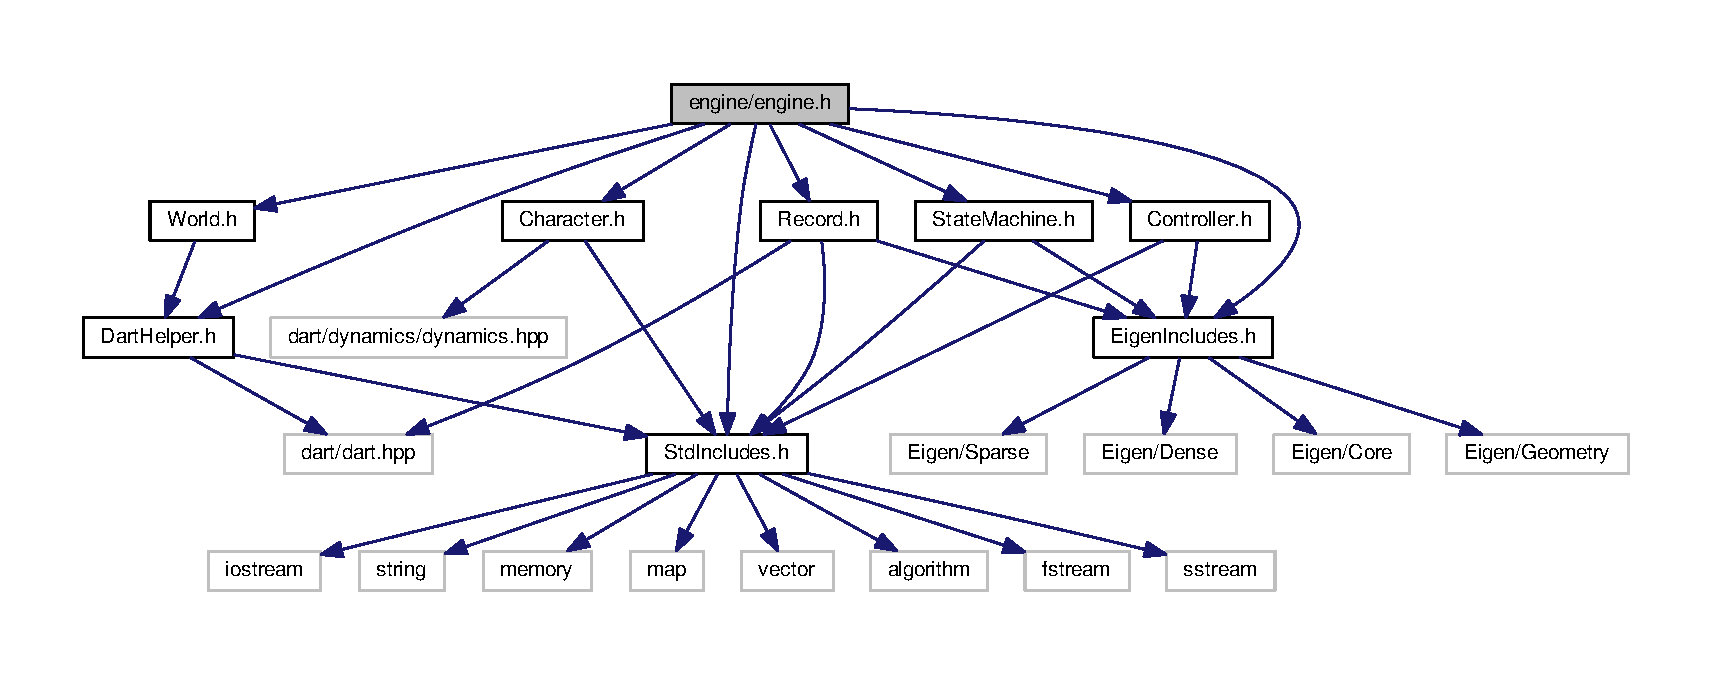
\includegraphics[width=350pt]{engine_8h__incl}
\end{center}
\end{figure}
Šis grafs rāda kuri faili tieši vai netieši iekļauj šo failu\+:
\nopagebreak
\begin{figure}[H]
\begin{center}
\leavevmode
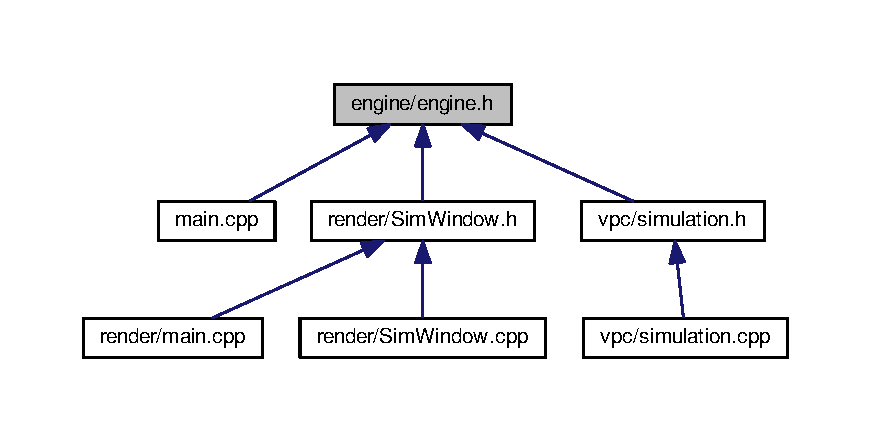
\includegraphics[width=350pt]{engine_8h__dep__incl}
\end{center}
\end{figure}
